\documentclass[letterpaper, 11pt]{article}

% set version variable
\newcommand{\versionnumber}{0.1}

% russian language
\usepackage[utf8]{inputenc}
\usepackage[T2A]{fontenc}
\usepackage[english, russian]{babel}
\usepackage{algorithmicx}
\usepackage{algpseudocode}
\usepackage{graphicx}

% math
\usepackage{amsmath}

\usepackage{amssymb} % some math symbols


% enumerate
\usepackage{enumerate}

% set type and margins of the page
\usepackage{geometry}  % document margins
\geometry{letterpaper, left=1.4in, right = 1.4in, top = 1.7in, bottom = 1.7in}

% color links in content
\usepackage{hyperref}
\hypersetup{
    colorlinks=true,
    linkcolor=red,
    urlcolor=blue,
    linktoc=all
}

% indent at first \par after section
\usepackage{indentfirst}

% fixed table and figures in section
\usepackage{float}

% colors
\usepackage{color}
\usepackage[usenames,dvipsnames]{xcolor}

% paragraph indent
\setlength{\parskip}{0.5em}

\title{\large{Краткий конспект}\\
\LARGE{Лекция 2. Выравнивание. Алгоритм Нидлмана-Вунша}\\
\normalsize версия \versionnumber (\textcolor{NavyBlue}{незавершенная})}
\date{18 февраля, 2016}
\author{Д. Ищенко\thanks{МФТИ} \and Б. Коварский\footnotemark[1]
\and И. Алтухов\footnotemark[1] \and Д. Алексеев\footnotemark[1]}

\begin{document}
\maketitle
\thispagestyle{empty}
\clearpage

% let's go
\section{Сравнение последовательностей}

В прошлом семестре мы говорили, что многие свойства биологических последовательностей можно выяснить "по гомологии", сравнивая их с другими последовательностями, чьи свойства нам уже известны. Но чтобы сравнивать нужно задать расстояние на строках. Если строки одинаковой длины, то можно подсчитать количество несовпадений, "мисматчей" в двух строках. Тогда мы получим расстояние Хэмминга:

$$d_H(V^l, W^l)=\sum_{i=1}^l[v_i\ne w_i]$$

$$V^l=(v_1,\ldots,v_l);\quad W^l=(w_1,\ldots,w_l)$$

Квадратные скобки в записи $[P]$ - это скобки Айверсона, переводящие истинное утверждение $P$ в $1$ и ложное в $0$. Здесь и далее придерживаемся следующих обозначений: $V^l$ - строка длины $l$, $v_i$ - символ в строке $V^l$ в позиции $i$, $V^j$ - префикс длины $j\le l$.

Ричард Хэмминг ввел такую меру для сравнения двоичных кодов. Ограниченное применение оно находит и в биоинформатике. Возможность сравнения строк лишь одинаковой длины - серьезное ограничение. Для того чтобы мы могли сравнивать строки разной длины помимо замены символа нужно добавить две других элементарных операции, вставку и удаление, возможность индела (insertion-deletion). Тогда мы сможем выравнить две последовательности, т.е. путем элементарных операций привести их к одинаковому виду. Оптимальное выравнивание минимизирирует количество таких элементарных операций над строками.

\begin{figure}[H]
  \center{
  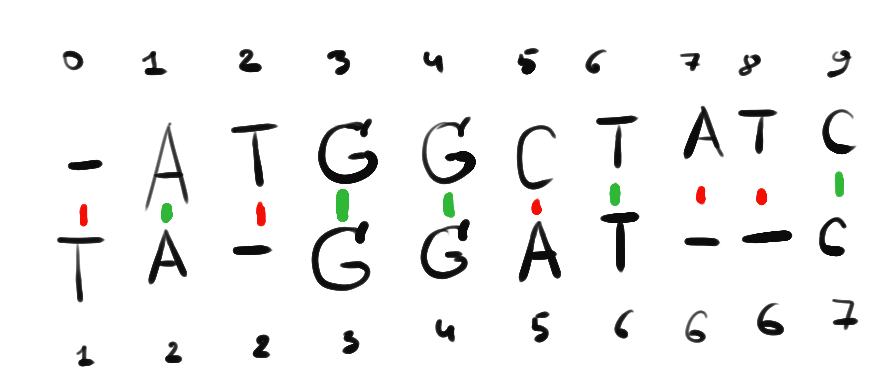
\includegraphics[scale=0.3]{fig/alignment_example.png}
  }
  \caption{Пример выравнивания последовательностей $\mathrm{ATGGCTATC}$ и $\mathrm{TAGGATC}$. Зеленым показаны совпадающие символы в выравнивании}
\end{figure}


Неформально же, выравнить две последовательности - записать их друг под другом, в некоторых местах допуская разрыв, так чтобы последовательности частично совпали друг с другом. Разрыв обычно обозначают дефисом. Возможность разрыва позволяет нам ровнять последовательности разной длины. Если рассуждать в терминах элементарных операций на строках, разрыв в одной последовательности означает, что в этой последовательности нам нужно сделать вставку символа чтобы перевести ее в другую.

Расстояние между двумя последовательностями равное минимальному числу элементарных операций, необходимых для перевода одной строки в другую - расстояние Левенштейна, $d_L$. Владимир Левенштейн ввел данную метрику на строках в 1965 году, как и Хэмминг, работая с двоичными кодами. Расстояния Левенштейна хорошо подходит для сравнения биологических последовательностей, потому что включает в себя биологическую подоплеку. Элементарные операции над строками соответствует эволюции последовательностей.

Если помимо вставки, удаления и замены допустить транспозицию (перестановку двух подряд идущих символов), то получим модифицированную функцию - расстояние Дамерау-Левенштейна. Оно часто используется в компьютерной лингвистике, в вычислительной биологии - редко.

Вернемся к выравниваниям. Давайте пронумеруем позиции в выравнивании. Тогда можно заметить, что любому выравниванию можно сопоставить некоторую последовательность точек на двумерной целочисленной решетке. Переходы из одного узла решетки в другой будут соответствовать элементарные операция над строками: движение по вертикали и горизонтали - вставки-удаления, по диагонали - замены (в случае, когда символы в строках отличаются). Направленно соединив каждый узел с определенными соседями, мы получим редакционный граф (edit graph). Выравниванию двух строк длины $n$ и $m$ будет соответствовать пути в этом направленном ациклическом графе из истока, вершины $(0,0)$ в сток, вершину $(n,m)$. Ребра в данном графе имеют вес - штрафы за несовпадения, если таковые имеются, и вставку. Пока считаем все штрафы равными единице.

\begin{figure}[H]
  \center{
  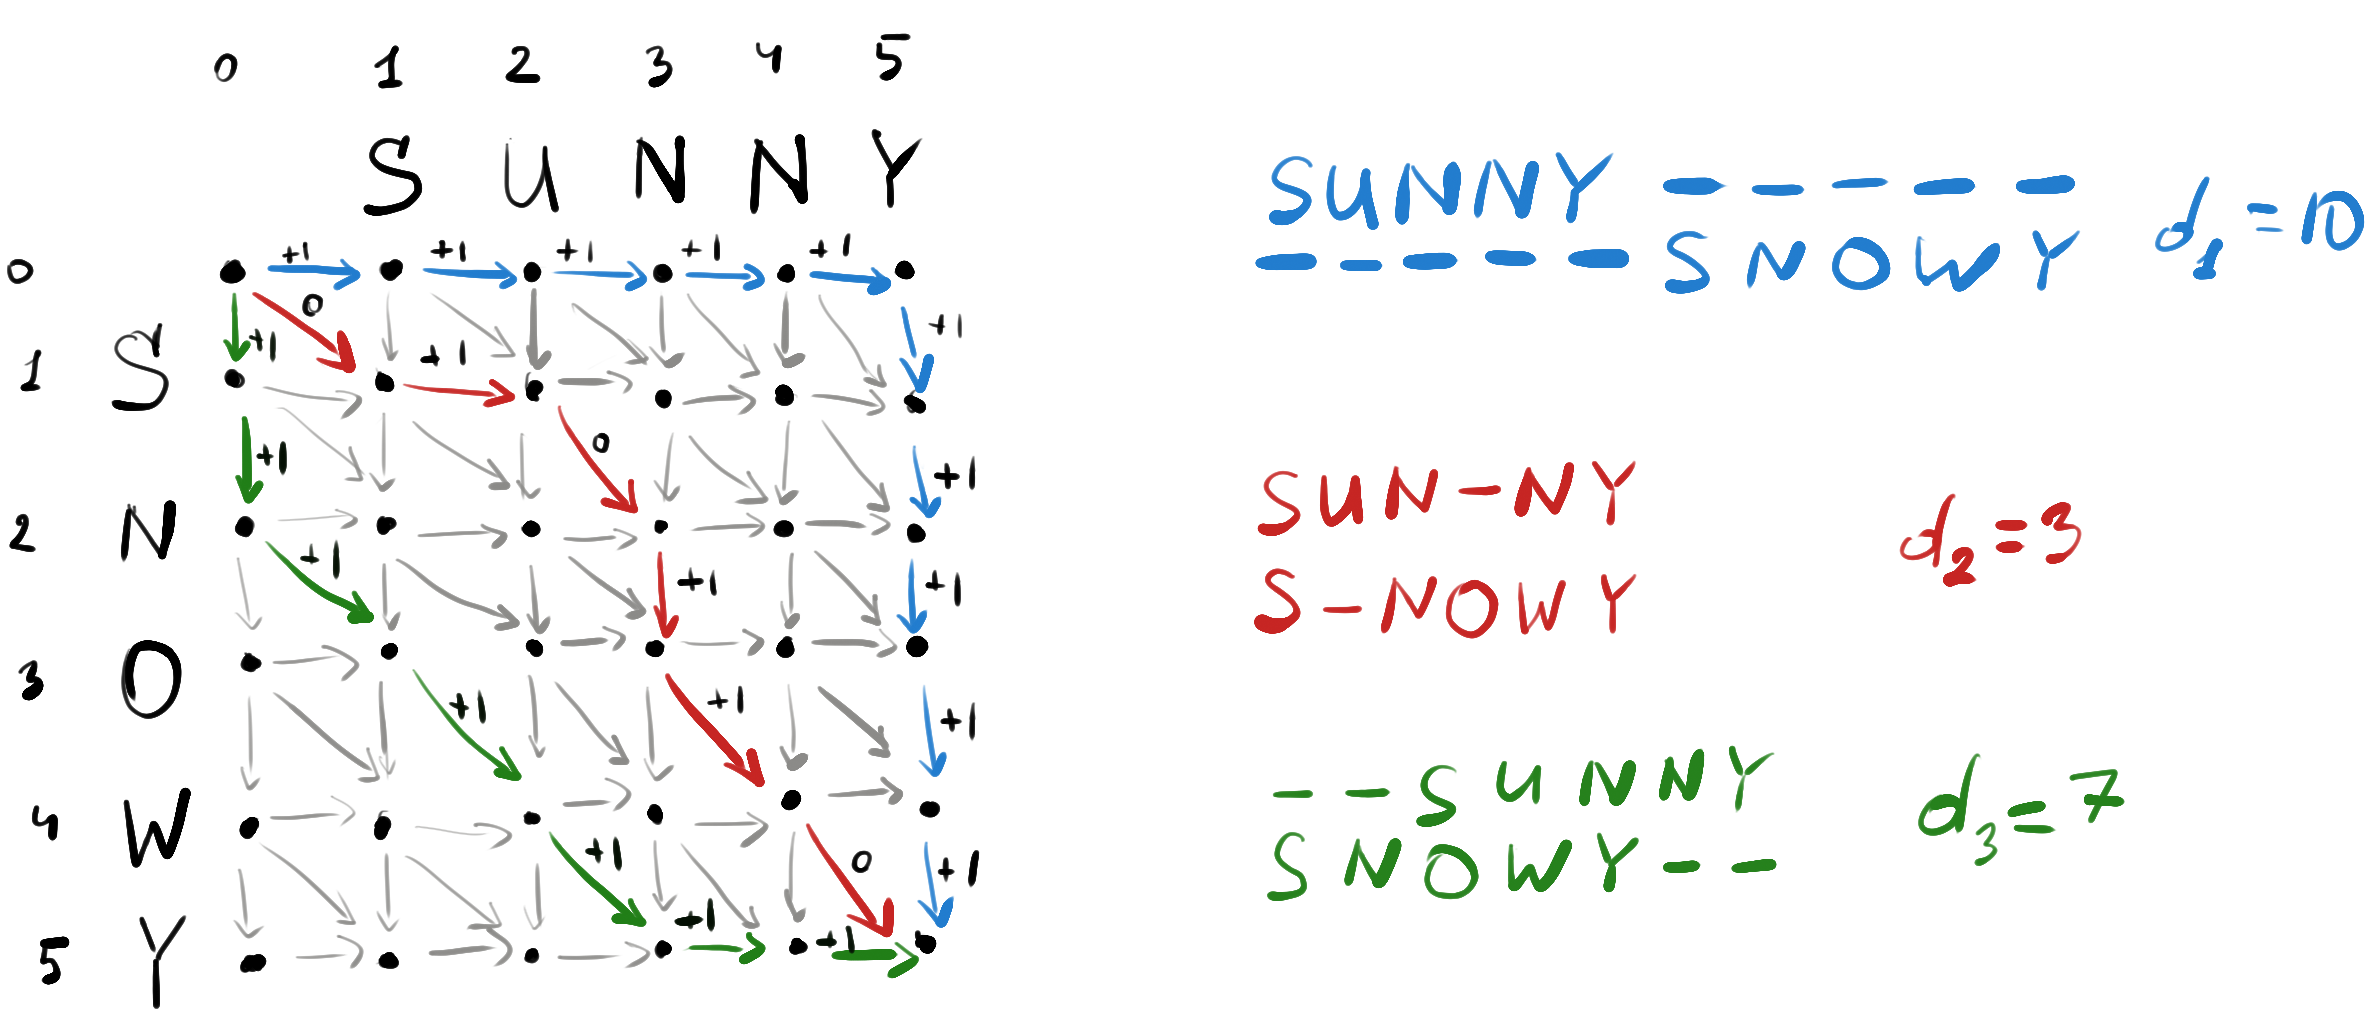
\includegraphics[scale=0.2]{fig/alignment_cases2.png}
  }
  \caption{Редакционный граф для последовательностей SUNNY и SNOWY. Трем путям из $(0,0)$ в $(5,5)$ соответствуют три выравнивания с разными редакционными расстояниями $d_1,d_2,d_3$.}
\end{figure}

Чтобы узнать редакционное расстояние (количество элементарных операций) для некоторого выравнивания достаточно просуммировать вес всех ребер, входящих в путь соответствующий данному выравниванию. Значит, оптимальное выравнивание - путь из стока в сток с наименьшим суммарным весом ребер.

Что если перебрать всевозможные пути в графе, попутно определяя их вес?

Давайте оценим снизу количество путей из $(0,0)$ в $(n,m)$, допуская лишь движения по вертикали и горизонтали. Любой такой путь можно закодировать двоичной последовательностью из $n$ единичек и $m$ нулей. Тогда количество таких путей равно $C^n_{m+n}$.

Считая $n\approx m >> 1$:

$$C_{2n}^n \approx \frac{(2n)!}{n!n!}\approx
\frac{\sqrt{4\pi n} (\frac{2n}{e})^{2n}}
 {(\sqrt{2\pi n} (\frac{n}{e})^{n})^2}=
\frac{\sqrt{4\pi n} (\frac{2n}{e})^{2n}}
 {2\pi n(\frac{n}{e})^{2n}}=\frac{2^{2n}}{\sqrt{\pi n}}
$$

Точное же количество выравниваний с учетом движения по диагонали:

$$N(n,m)=\sum_{k=0}^{\min (n,m)}2^k C^k_m C^k_n$$

Экспоненциальная сложность алгоритма - очень плохой результат. Нужен иной подход. Во-первых, заметим, что расстояние Левенштейна симметрично:

$$d_L(W^m, V^n)=d_L(V^n, W^m)$$

Во-вторых, если одна из строк пустая, расстояние Левенштейна равно длине ненулевой.

$$d_L(0, V^n)=n$$
$$d_L(0, 0)=0$$


Теперь рассмотрим вершину $(i,j)$ в редакционном графе. Наименьший вес пути из вершину $(0,0)$ в $(i,j)$ равен расстоянию Левенштейна между префиксами $V^i$ и $W^j$. В вершину $(i,j)$ мы могли прийти лишь тремя способами: из $(i-1,j)$ по горизонтали (при этом мы сделали разрыв в строке $V$, пройдя по ребру с весом 1), из $(i,j-1)$ по вертикали (при этом мы сделали разрыв в строке $W$, пройдя по ребру с весом 1), либо из $(i-1,j-1)$ по диагонали. Вес такого ребра равен $0$, если $v_i=w_j$ и равен $1$, если $v_i\ne w_j$. Из трех возможных переходов мы должны выбрать такой, который бы минимизировал суммарный вес. Тогда:

$$d_L(V^i,W^j) = \min
	\begin{pmatrix} d_L(V^{i-1},W^j)+1, \\
	 d_L(V^{i},W^{j-1})+1, \\
	 d_L(V^{i-1}_1,W^{j-1})+[v_i\ne w_j]
	 \end{pmatrix},\quad \quad i\ne 0 \land j\ne 0\\
$$

В итоге мы записали рекурсивную формулу для расстояния Левенштейна. Видно, чтобы вычислить значение в вершине $(i,j)$ нам нужно знать редакционное расстояния лишь в вершинах $(i-1,j-1)$, $(i-1,j)$, $(i,j-1)$.
Рекурсивная структура расстояния, подсказывает, что эту задачу можно эффективно решить при помощи динамического программирования.

Динамическое программирование - способ решения задач путем их разбиения их на более простые подзадачи. Стоит заметить, этот термин родом не из компьютерных наук, а из теории оптимизации. Автор "динамического программирования", Ричард Беллман, под программированием понимал не написание программ, "планирование" многоступенчатых процессов.

Чтобы лучше понять смысл динамического программирования, рассмотрим три задачи, нахождения факториала, биномиального коэффициента и числа Фибоначчи. Что в них общего? Все три величины можно задать рекурсивно.

$$n!=n*(n-1)!;\quad 1!=1$$
$$C^k_n=C^k_{n-1} + C^{k-1}_{n-1};\quad C^0_n=1, C^n_n=1$$
$$F_n=F_{n-1}+F_{n-2};\quad F_1=1, F_2=1$$

Поэтому процесс вычисления можно изобразить в виде направленного ациклического графа.

\begin{figure}[H]
  \center{
  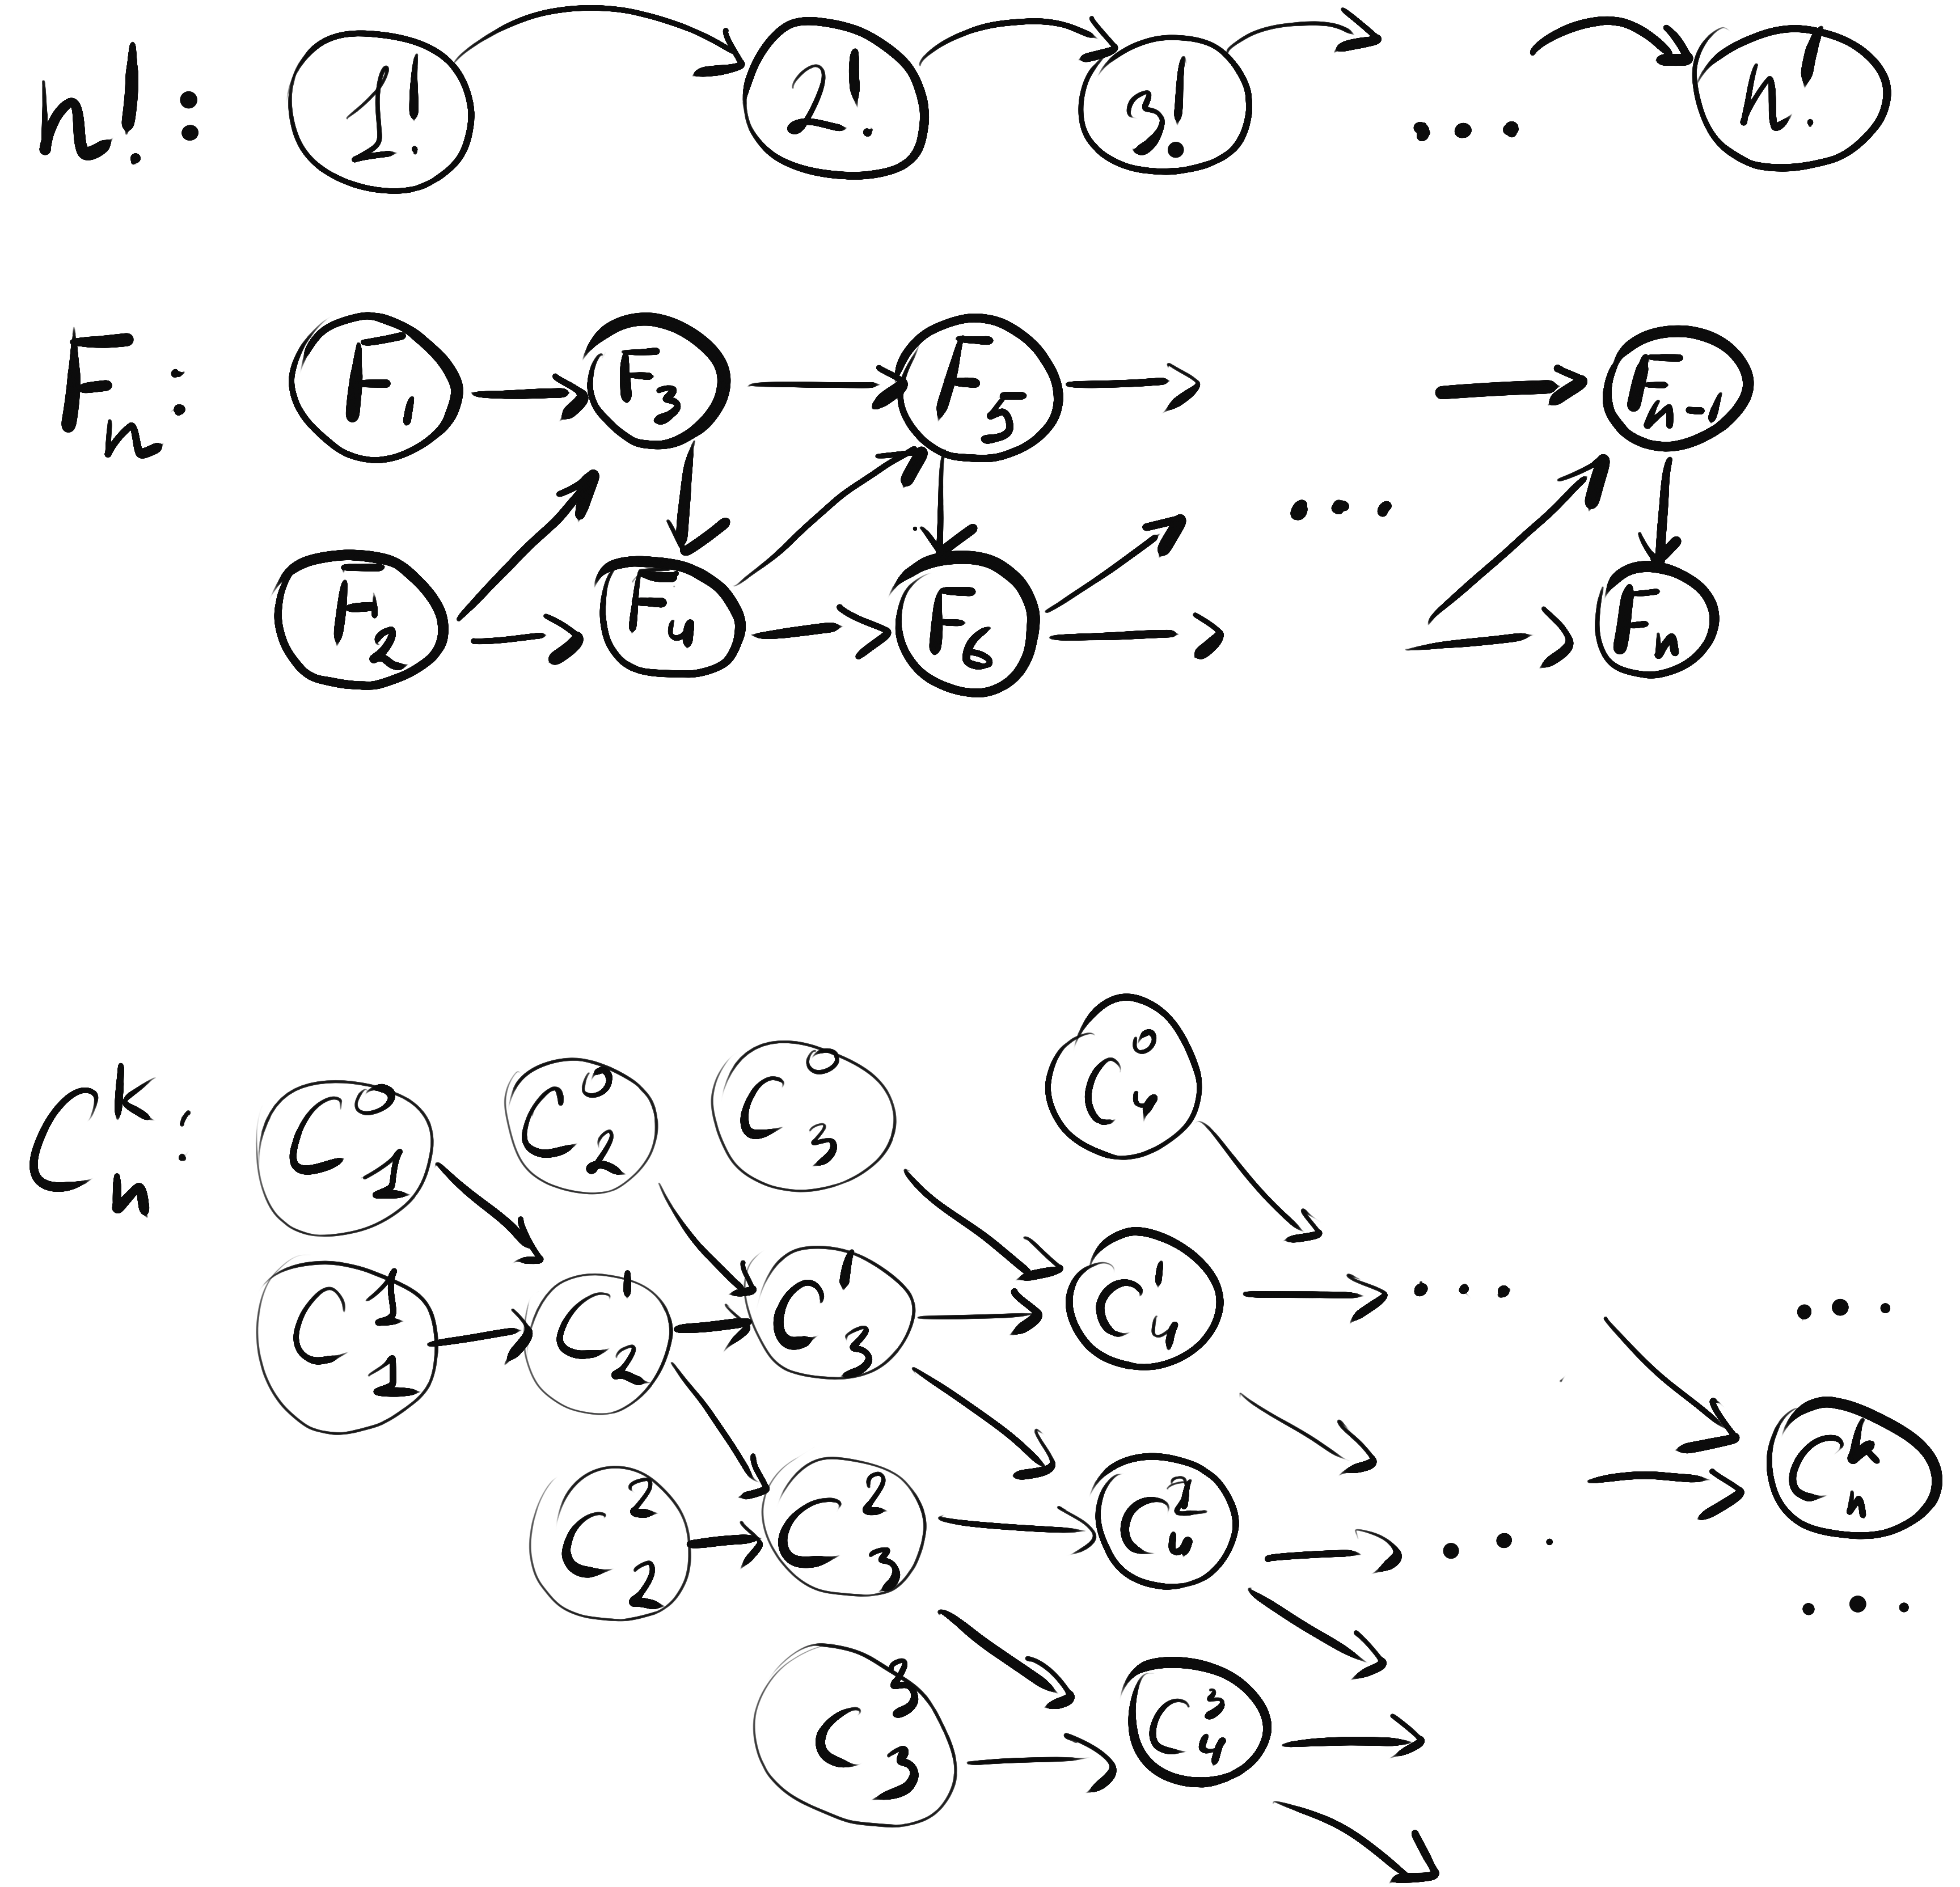
\includegraphics[scale=0.1]{fig/dynamic_routines.png}
  }
  \caption{Графы подзадач для нахождения значений факториала, числа Фибоначчи и биномиального коэффициента}
\end{figure}

Но просто написать рекурсивную функцию для их вычисления будет неэффективно. Скажем, в задаче про числа Фибоначчи при рекурсивном вызове нам придется многократно вычислять промежуточные значения и сложность будет экспоненциальной. Вместо этого мы можем решать задачу снизу-вверх, запоминая промежуточный результат и используя уже вычисленное значения во всех последующих обращениях. Тогда сложность вычисления числа Фибоначчи будет $O(n)$.

Давайте вернемся к нашему графу. В вершинах графа, по сути в таблице размера $(n+1) \times (m+1)$ можно хранить промежуточный результат - величину расстояние Левенштейна, равное сумме весов ребер кратчайшего пути в эту вершин.

\begin{figure}[H]
  \center{
  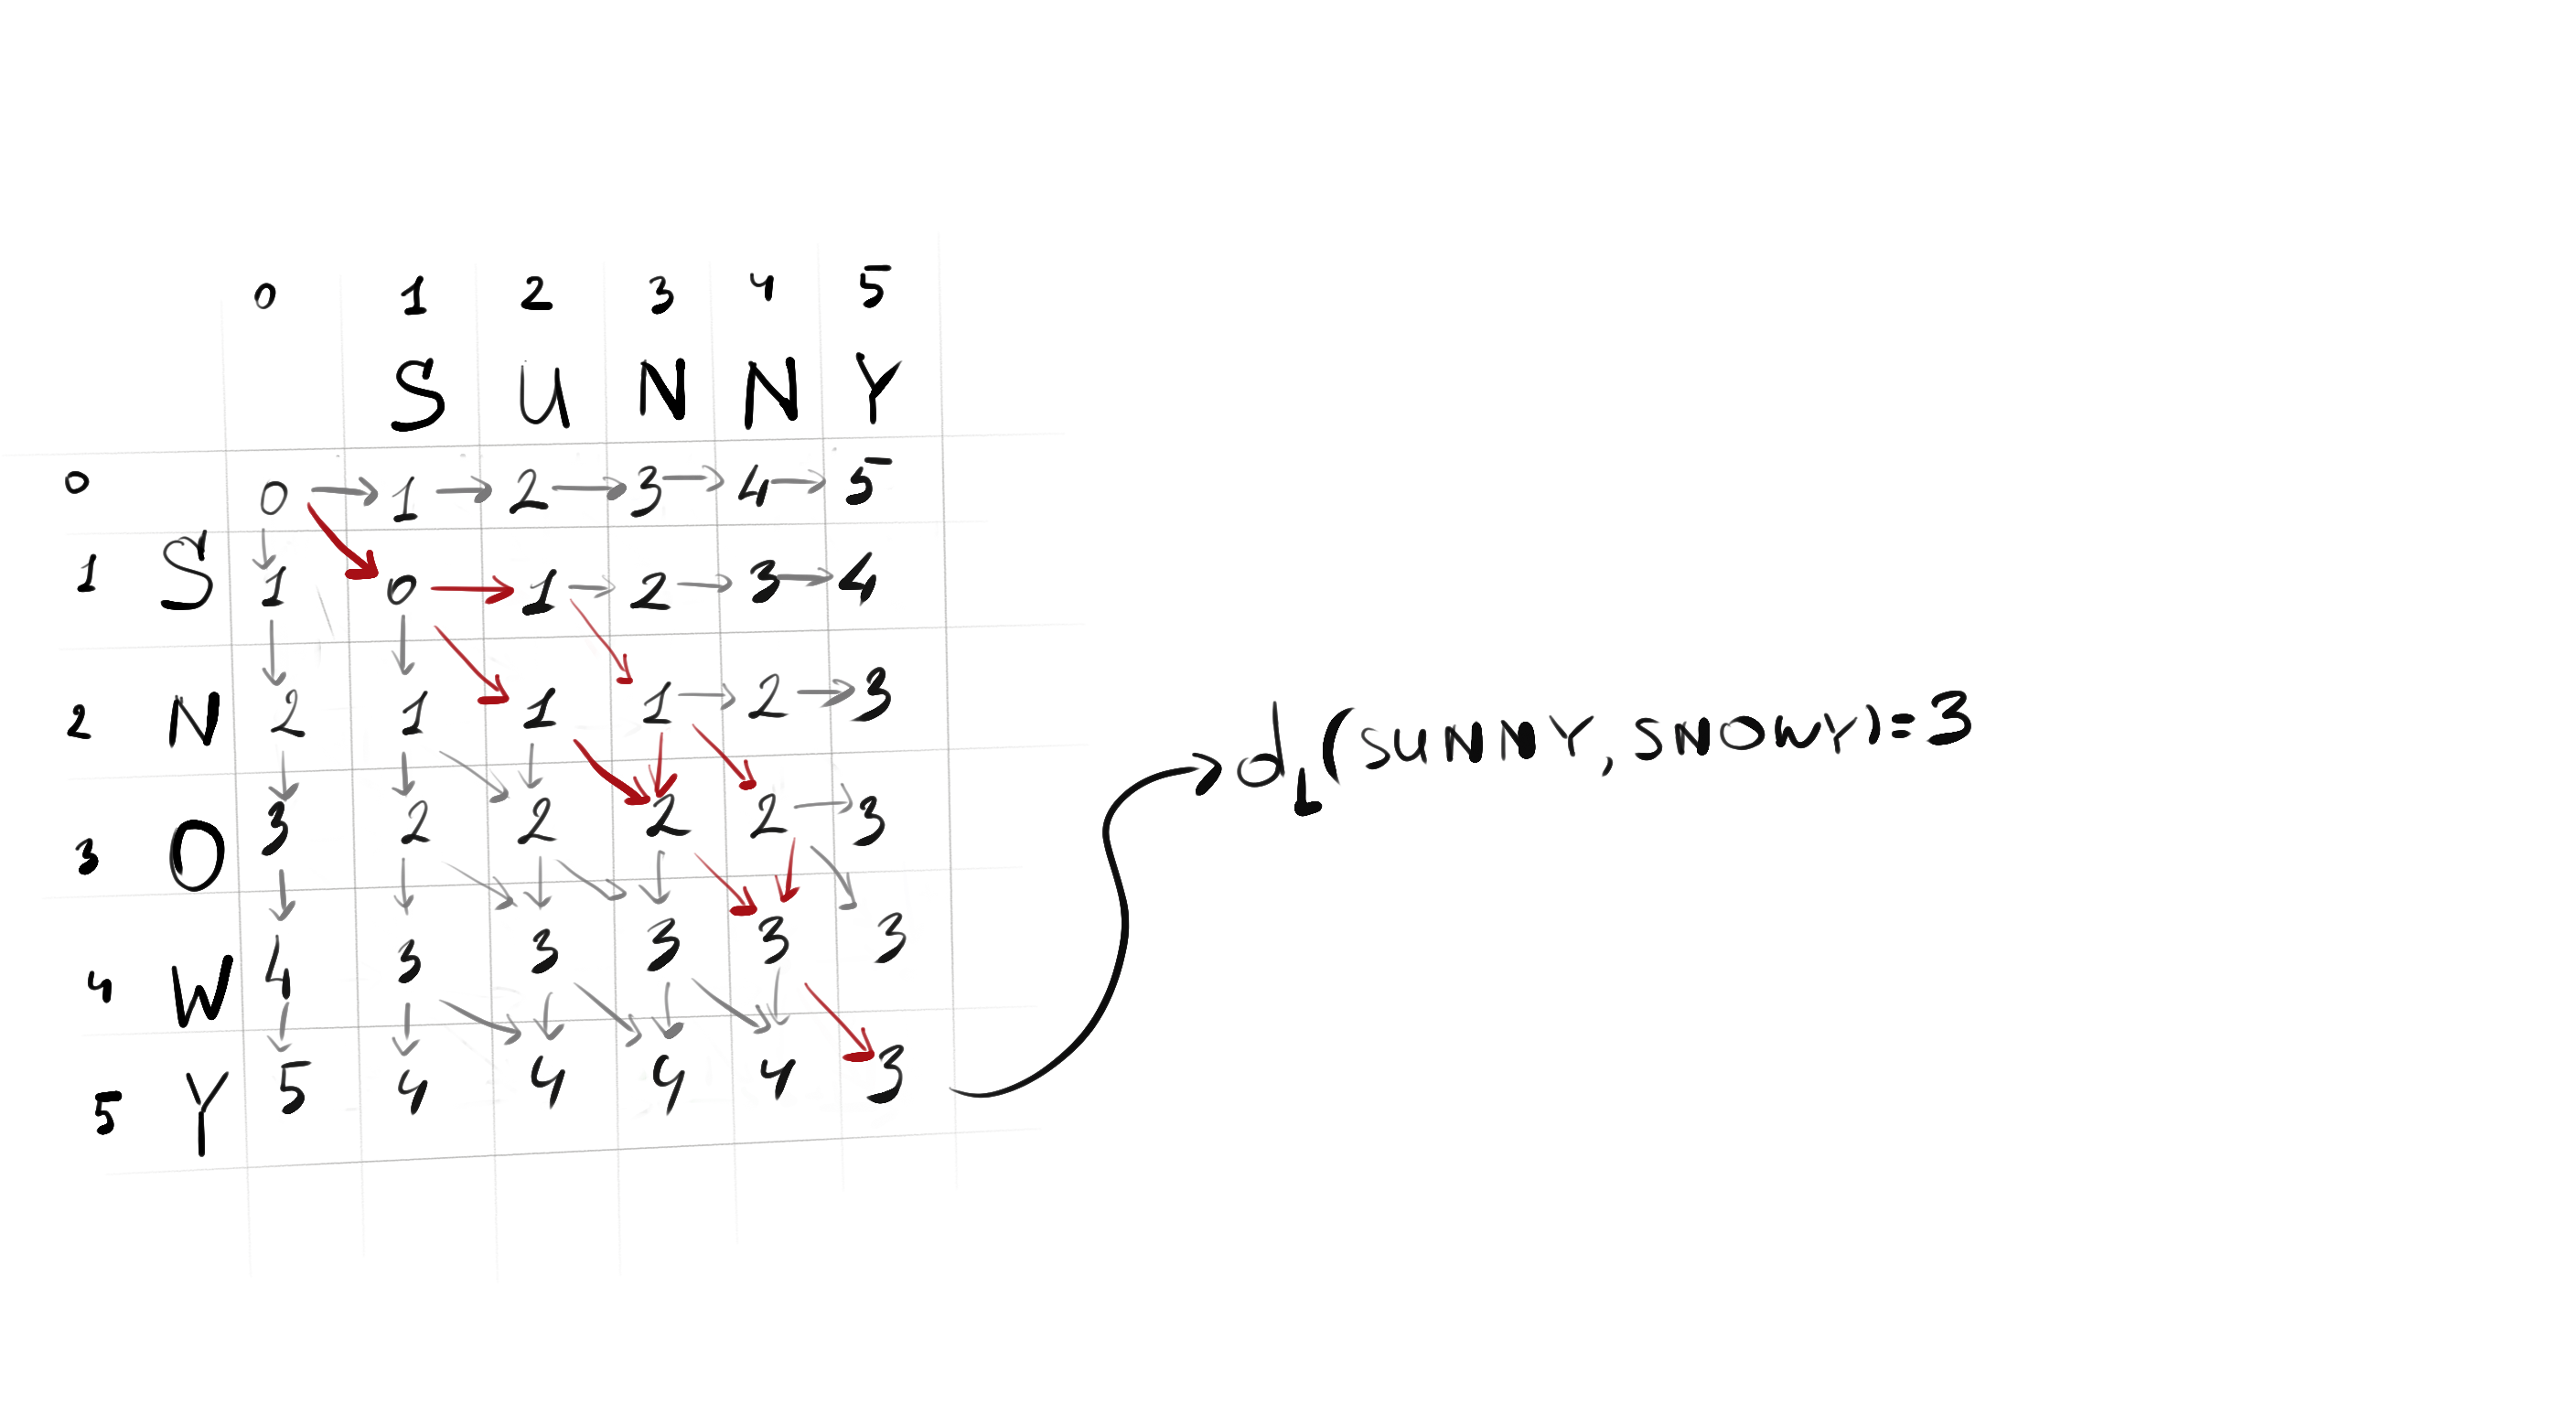
\includegraphics[scale=0.2]{fig/edit_distances.png}
  }
  \caption{Таблица со значениями расстояний Левенштейна для строк SNOWY и SUNNY с направлениями оптимальных переходов. Красным показан путь, соответствующий оптимальному выравниванию}
\end{figure}

Напишем код нахождения редакционного расстояния и заполнения таблицы:

\begin{algorithmic}[1]
\Procedure{LevensteinDistance}{$V,W$}
\State $D\gets [\quad]$\Comment{Создаем массив для хранения расстояний}
\For{$i\gets 0, n$}\Comment{$n$ - длина первой последовательности}
\State $D[i,0]\gets i$
\EndFor

\For{$j\gets 0, m$}\Comment{$m$ - длина второй последовательности}
\State $D[0,j]\gets j$
\EndFor

\For{$i\gets 1, n$}
\For{$j\gets 1, m$}
\State $D[i,j]\gets
\min
\begin{pmatrix} D[i-1,j]+1, \\
	 D[i,j-1]+1, \\
	 D[i-1,j-1]+(V[i]\ne W[j])
\end{pmatrix}$
\EndFor
\EndFor
\State \textbf{return} $D$
\EndProcedure
\end{algorithmic}

Для того чтобы восстановить по таблице редакционных расстояний само выравнивание нам необходимо помнить каким образом мы попали в вершину. Помимо таблицы с редакционными расстояниями следует завести таблицу (backtracker), где бы хранились направления переходов:

\begin{algorithmic}[2]
\Procedure{NWGlobalAlignment}{$V,W$}
\State $D\gets [\quad]$
\State $B\gets [\quad]$\Comment{Создаем массив для хранения направлений}
\For{$i\gets 0, n$}
\State $D[i,0]\gets i$
\State $B[i,0]\gets "\rightarrow"$
\EndFor

\For{$j\gets 0, m$}
\State $D[0,j]\gets j$
\State $B[0,j]\gets "\downarrow"$
\EndFor

\For{$i\gets 1, n$}
\For{$j\gets 1, m$}

\State $D[i,j]\gets D[i-1,j-1]+(V[i]\ne W[j])$
\State $B[i,j]\gets "\searrow"$

\If{$D[i,j]>D[i-1,j]+1$}
\State$D[i,j]\gets D[i-1,j]+1$
\State $B[i,j]\gets "\rightarrow"$
\EndIf

\If{$D[i,j]>D[i,j-1]+1$}
\State$D[i,j]\gets D[i,j-1]+1$
\State $B[i,j]\gets "\downarrow"$
\EndIf

\EndFor
\EndFor
\State \textbf{return} $B$
\EndProcedure
\end{algorithmic}

Итак, подведем итоги. Мы построили разобрали алгоритм Нидлмана-Вунша, который позволяет находить расстояние Левенштейна между двумя строками и тем самым строить оптимальное глобальное выравнивание. Сложность такого алгоритма $O(nm)$, затраты по памяти также $O(nm)$.

Но этого еще недостаточно. Нам хотелось бы выравнивать биологические последовательности и хочется чтобы у расстояний была какая-то биологическая основа. Поэтому в биологических приложениях обычно делают иначе, вместо задачи минимизации редакционного расстояния, решая задачу максимизации сходства, очков выравнивания. При этом, за совпадение награждают, а за несовпадения и вставки и удаления штрафуют. При этом штраф за индел зависит от его размера, штраф за несовпадения зависит от типа замены. Об этом на следующей лекции.

\section{Ссылки}
\begingroup
\renewcommand{\section}[2]{}%
\begin{thebibliography}{7}
\bibitem{Frank}
Gusfield D. Algorithms on strings, trees and sequences: computer science and computational biology. – Cambridge university press, 1997.
\bibitem{Frank}
Дасгупта С., Пападимитриу Х., Вазирани У. Алгоритмы – Издательство МЦНМО, 2014.
\bibitem{Frank}
Jones N., Pevzner P. An Introduction to Bioinformatics Algorithms – MIT Press, 2004.
\end{thebibliography}


\end{document} 